\chapter{Anforderungen}

Dieses Kapitel beginnt mit einer Recherche über die aktuellen Prozesse 
eines Notfalleinsatzes und untersucht, an welcher Stelle der Einsatz von 
Telemedizin bereits angedacht oder in vereinfachter Form bereits in Betrieb ist. 
Die recherchierten Informationen wurden im Rahmen dieser 
Arbeit ermittelt und spiegeln den aktuellen Stand wider. 
Darüber hinaus werden die Erwartungen an die Anwendung 
aufgezeigt und in funktionale und nicht-funktionale 
Anforderungen aufgeteilt sowie thematisiert. Abschließend 
erfolgt eine Präzisierung der Anforderungen.

\section{Aktueller Stand Notfalleinsatz}

In Deutschland beginnt ein Notfalleinsatz, wie etwa bei einem gestürzten 
Patienten, mit einem Anruf bei der Notrufnummer 112. 
Der Anrufer beschreibt die Situation, und die 
Einsatzleitstelle bewertet diese Informationen, 
um angemessene Rettungskräfte zu entsenden. Sobald die 
Rettungskräfte am Einsatzort eintreffen, beurteilen sie 
den Gesundheitszustand des Patienten. Sie leisten Erste 
Hilfe und stabilisieren den Patienten. Dabei werden 
eventuelle Verletzungen versorgt, Vitalfunktionen 
kontrolliert und bei Bedarf lebensrettende Maßnahmen 
durchgeführt. Bei Bedarf wird der Patient anschließend in 
ein Krankenhaus transportiert, um eine weiterführende 
medizinische Versorgung zu gewährleisten. Jede Maßnahme 
wird sorgfältig entsprechend der medizinischen 
Dringlichkeit und der spezifischen Situation des Patienten 
ausgewählt und durchgeführt.\\

\begin{figure}[H]
    \centering
    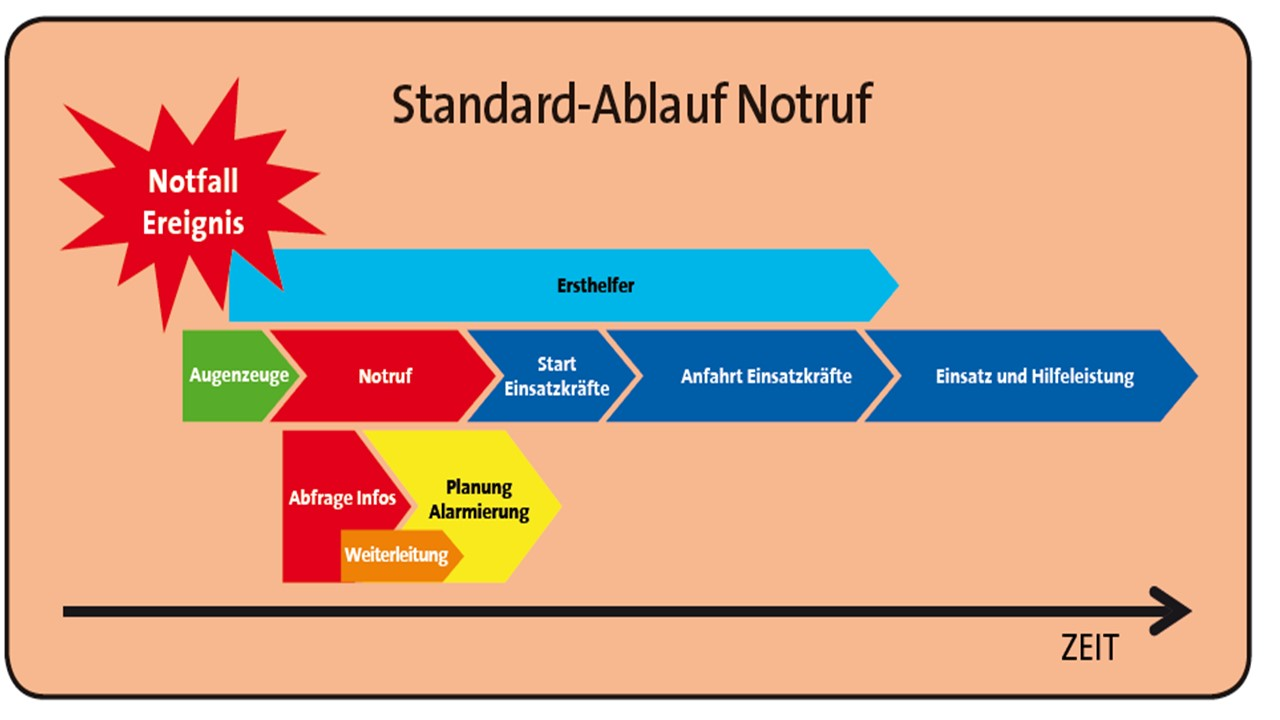
\includegraphics[width=1.0\textwidth]{Ablauf_Notruf}
    \caption{Abbildung eines Notfalleinsatzes.[Quelle: \cite{NotfallAblauf}]}
    \label{img:Ablauf_Notruf}
\end{figure}


Beim Zusammenspiel von Notfallsanitätern und Notärzten in 
Deutschland ergänzen sich beide Berufsgruppen. 
Notfallsanitäter treffen zuerst am Einsatzort ein, 
leisten Erste Hilfe und beginnen mit der Patientenversorgung. 
Sie haben eine umfassende Ausbildung und dürfen bestimmte 
medizinische Maßnahmen eigenständig durchführen. Wenn die 
Situation des Patienten es erfordert, wird zusätzlich ein Notarzt hinzugezogen. 
Dieser kann erweiterte medizinische Maßnahmen vornehmen, wie zum 
Beispiel das Verabreichen bestimmter Medikamente oder invasive Eingriffe. 
Gemeinsam stellen Notfallsanitäter und Notarzt die bestmögliche 
Versorgung des Patienten sicher.\\


Der Einsatz einer entfernten Unterstützung durch einen Notarzt, wie 
zum Beispiel telefonische Beratung, wird derzeit nicht 
praktiziert. Dies liegt unter anderem an Herausforderungen 
wie eingeschränkter Sprachqualität, Verständnisproblemen 
und rechtlichen Unsicherheiten bezüglich der Delegation 
medizinischer Maßnahmen. 

\section{Erwartungen an die TNA-Software}

Die Erwartungen an eine präklinische Telenotarzt-Software sind vielfältig.

Eine solche Software sollte eine intuitive Benutzeroberfläche besitzen, die selbst unter Stressbedingungen einfach zu bedienen ist. Ihre Funktionalität muss auf verschiedenen Geräten wie Tablets, Smartphones und Pc's gewährleistet sein, um eine breite Zugänglichkeit zu ermöglichen. Ein Kernaspekt der Software ist die Bereitstellung einer stabilen und sicheren Kommunikationsverbindung, die eine Video- und Audiokommunikation zwischen dem Telenotarzt und dem Rettungsdienstpersonal ermöglicht. Hierbei ist die Qualität der Übertragung entscheidend, um Fehldiagnosen und Missverständnisse zu vermeiden.

Wichtig ist auch die Fähigkeit der Software, patientenbezogene Daten effizient zu erfassen, zu speichern und zu verarbeiten. Dies umfasst Vitalparameter, Medikamentenlisten und Allergieinformationen.

Der Datenschutz und die Sicherheit der übertragenen medizinischen Daten haben oberste Priorität. Verschlüsselung der Datenübertragung und strenge Zugriffskontrollen sind unerlässlich, um die Privatsphäre der Patienten zu schützen. Zudem sollte die Software mit anderen medizinischen Systemen und Geräten interoperabel sein und eine flexible Architektur aufweisen, die Anpassungen an lokale Gegebenheiten und zukünftige technologische Entwicklungen ermöglicht.


\section{Anforderungsanalyse}


Dieses Kapitel widmet sich der ausführlichen Darstellung der verschiedenen Anforderungsarten der Applikation. 
Zunächst wird der Anwendungsfall durch ein aussagekräftiges Diagramm visualisiert. Im Anschluss daran folgt eine Erläuterung der User-Stories, 
die als Grundlage für die Ableitung der funktionalen Anforderungen dienen. Nachfolgend werden die nicht-funktionalen Anforderungen aufgeführt und detailliert 
beschrieben. Sowohl die funktionalen als auch die nicht-funktionalen Anforderungen werden in übersichtlichen Tabellen präsentiert, die eine klare Priorisierung 
und Zusammenfassung der einzelnen Punkte ermöglichen. Das Kapitel schließt mit einer präzisen Abgrenzung der Anforderungen ab, die als Orientierung für die 
nachfolgenden Kapitel dient.


\subsection{Use-Cases der TNA-Software}

Im Folgenden werden zwei Use-Cases für die TNA-Software präsentiert, um deren Funktionalitäten und Anwendungsgebiete genauer zu erläutern und zu vertiefen. \\\\

\textbf{Use-Case 1:} Alamierung für den Telenotarzt \\

Dieser Use-Case konzentriert sich auf die Anwendung der TNA-Software zur Optimierung des Einsatzablaufs für Notfallsanitäter im präklinischen Bereich.

\textbf{Akteure}\\

\begin{itemize}
    \item Notfallsanitäter
    \item Telenotarzt
\end{itemize}

\textbf{Hauptablauf}\\


\begin{enumerate}
\item Der Notfallsanitäter erhält einen Einsatzauftrag von der Rettungsleitstelle.
\item Während der Anfahrt zum Einsatzort verwendet der Sanitäter eine Dokumentationssoftware, um Echtzeitinformationen über den Einsatzort, die Patientenhistorie und eventuelle spezielle Anforderungen zu erhalten.
\item Die Software bietet die Möglichkeit, bei bedarf unterstützung eines TNA anzufordern.
\item Bei angeforderter unterstützung, werden sämtliche Patientendaten, Vitalzeichen und Symptomen an die TNA Software übermittelt.
\item Aufgrundlage der informationen, werden in der TNA-Software handlungsanweisungen geladen.
\item Während des Einsatzes kann der TNA auf medizinische Referenzdaten und Protokolle über die Software zugreifen.
\item Nach der Patientenversorgung und dem Transport zum Krankenhaus erfolgt die digitale Dokumentation des Einsatzes über die TNA-Software.
\end{enumerate}


\textbf{Alternativablauf}\\
Bei Bedarf kann die Software in Echtzeit auf Änderungen in der Einsatzsituation reagieren und Vorschläge für alternative Behandlungsmaßnahmen oder den Transport zu einem speziellen Krankenhaus geben.\\

\textbf{Use-Case 2:} Virtuelle Arztkonsultation \\

Dieser Use-Case beschreibt, wie die TNA-Software eine virtuelle Arztkonsultation während eines Rettungseinsatzes ermöglicht.

\textbf{Akteure}\\

\begin{itemize}
    \item Notfallsanitäter
    \item Telenotarzt
\end{itemize}

\textbf{Hauptablauf}\\

\begin{enumerate}
\item Während eines komplexen Einsatzes mit unklarer Diagnose oder speziellen medizinischen Herausforderungen aktiviert der Notfallsanitäter die virtuelle Arztkonsultation über die TNA-Software.
\item Die Software stellt eine sichere WebRTC-Verbindung zwischen dem Notfallsanitäter vor Ort und einem bereitstehenden Fernarzt her.
\item Der Telenotarzt kann live über die in den Rettungsfahrzeugen installierten Kameras und die mobilen Geräte der Sanitäter auf die Einsatzsituation zugreifen.
\item Der Telenotarzt kann den Notfallsanitäter bei der Diagnosestellung, der Auswahl von Behandlungsmaßnahmen und der Entscheidung über den weiteren Verlauf des Einsatzes unterstützen.
\item Die TNA-Software ermöglicht die gemeinsame Nutzung von medizinischen Daten und Befunden in Echtzeit.
\item Nach Abschluss der virtuellen Konsultation und Behandlungsempfehlungen kann der Einsatz vor Ort fortgesetzt werden. 
\end{enumerate}

\textbf{Alternativablauf}\\
- Bei Bedarf kann die TNA-Software auch eine Übertragung von Vitaldaten und medizinischen Bildern an den Telenotarzt ermöglichen, um eine fundierte Diagnose zu erleichtern.\\

Diese erweiterte Darstellung der beiden Use-Cases verdeutlicht die vielfältigen Anwendungsgebiete und den Nutzen der TNA-Software im Bereich der präklinischen Notfallversorgung. Die Software bietet nicht nur Unterstützung für Notfallsanitäter vor Ort, sondern ermöglicht auch eine effektive Zusammenarbeit mit Telenotarzt, um die bestmögliche Patientenversorgung sicherzustellen.


\subsection{Funktionale Anforderungen}
Funktionale Anforderungen in der Softwareentwicklung beschreiben Funktionen, Verhaltensweisen oder Leistungen, die eine Software oder ein System erbringen muss. 
Sie definieren, was das System tun soll, in verschiedenen Szenarien und unter verschiedenen Bedingungen. \cite{braun2016nicht}\\

\begin{itemize}
    \item \textbf{FA\#01} Die Anwendung muss die Möglichkeit bieten, sich sowohl als Notfallsanitäter als auch als Notarzt anzumelden.
    \item \textbf{FA\#02} Lorem ipsum dolor sit amet, consetetur sadipscing elitr, sed diam nonumy eirmod tempor invidunt ut labore et dolore magna aliquyam erat, sed diam voluptua. At vero eos et accusam et
    \item \textbf{FA\#03} Lorem ipsum dolor sit amet, consetetur sadipscing elitr, sed diam nonumy eirmod tempor invidunt ut labore et dolore magna aliquyam erat, sed diam voluptua. At vero eos et accusam et
    \item \textbf{FA\#04} Lorem ipsum dolor sit amet, consetetur sadipscing elitr, sed diam nonumy eirmod tempor invidunt ut labore et dolore magna aliquyam erat, sed diam voluptua. At vero eos et accusam et
    \item \textbf{FA\#05} Lorem ipsum dolor sit amet, consetetur sadipscing elitr, sed diam nonumy eirmod tempor invidunt ut labore et dolore magna aliquyam erat, sed diam voluptua. At vero eos et accusam et

\end{itemize}

\subsection{Nicht funktionaleAnforderungen}
Nicht-funktionale Anforderungen beziehen sich auf die allgemeine Qualität und Eigenschaften eines Systems, die nicht direkt dessen spezifische Funktionen betreffen. Sie beschreiben, wie gut ein System funktionieren soll und legen Standards fest. \cite{bergsmann2004nicht}

\begin{itemize}
    \item \textbf{NFA\#01} Die Anwendung muss die fähigkeit besitzen, mit steigender Nutzerzahl oder Datenvolumen effizient umzugehen.
    \item \textbf{NFA\#02} Lorem ipsum dolor sit amet, consetetur sadipscing elitr, sed diam nonumy eirmod tempor invidunt ut labore et dolore magna aliquyam erat, sed diam voluptua. At vero eos et accusam et
    \item \textbf{NFA\#03} Lorem ipsum dolor sit amet, consetetur sadipscing elitr, sed diam nonumy eirmod tempor invidunt ut labore et dolore magna aliquyam erat, sed diam voluptua. At vero eos et accusam et
    \item \textbf{NFA\#04} Lorem ipsum dolor sit amet, consetetur sadipscing elitr, sed diam nonumy eirmod tempor invidunt ut labore et dolore magna aliquyam erat, sed diam voluptua. At vero eos et accusam et
    \item \textbf{NFA\#05} Lorem ipsum dolor sit amet, consetetur sadipscing elitr, sed diam nonumy eirmod tempor invidunt ut labore et dolore magna aliquyam erat, sed diam voluptua. At vero eos et accusam et

\end{itemize}

\subsection{Zusammenfassung und Priorisierung}

In diesem Kapitel erfolgt eine strukturierte und übersichtliche Darstellung der verschiedenen Anforderungen an das Projekt, sowohl der funktionalen als auch der nicht-funktionalen Art. Diese Anforderungen werden in tabellarischer Form präsentiert, um eine klare und zugängliche Übersicht zu gewährleisten.



\begin{table}[ht]
    \centering
    \begin{tabularx}{\textwidth}{@{}lX@{}}
    \toprule
    ID & Funktionale Anforderung \\ 
    \midrule
    FA\#01 & Benutzeranmeldung \\
    FA\#02 & Lorem ipsum dolor sit amet \\
    FA\#03 & Lorem ipsum dolor sit amet \\
    FA\#04 & Lorem ipsum dolor sit amet \\
    FA\#05 & Lorem ipsum dolor sit amet \\
    \bottomrule
    \end{tabularx}
    \caption{Tabellarische Übersicht der funktionalen Anforderungen}
    \label{tab:FA-tabelle}
    \end{table}

\begin{table}[ht]
    \centering
    \begin{tabularx}{\textwidth}{@{}lX@{}}
    \toprule
    ID & Nicht-funktionale Anforderung \\ 
    \midrule
    NFA\#01 & Skalierbarkeit \\
    NFA\#02 & Lorem ipsum dolor sit amet \\
    NFA\#03 & Lorem ipsum dolor sit amet \\
    NFA\#04 & Lorem ipsum dolor sit amet \\
    NFA\#05 & Lorem ipsum dolor sit amet \\
    \bottomrule
    \end{tabularx}
    \caption{Tabellarische Übersicht der Nicht-funktionalen Anforderungen}
    \label{tab: NFA-tabelle}
    \end{table}

\subsection{EingrenzungenNFAAnforderungen}
Lorem ipsum dolor sit amet, consetetur sadipscing elitr, sed diam nonumy eirmod tempor invidunt ut labore et dolore magna aliquyam erat, sed diam voluptua. At vero eos et accusam et justo duo dolores et ea rebum. Stet clita kasd gubergren, no sea takimata sanctus est Lorem ipsum dolor sit amet. Lorem ipsum dolor sit amet, consetetur sadipscing elitr, sed diam nonumy eirmod tempor invidunt ut labore et dolore magna aliquyam erat, sed diam voluptua. At vero eos et accusam et justo duo dolores et ea rebum. Stet clita kasd gubergren, no sea takimata sanctus est Lorem ipsum dolor sit amet. Lorem ipsum dolor sit amet, consetetur sadipscing elitr, sed diam nonumy eirmod tempor invidunt ut labore et dolore magna aliquyam erat, sed diam voluptua. At vero eos et accusam et justo duo dolores et ea rebum. Stet clita kasd gubergren, no sea takimata sanctus est Lorem ipsum dolor sit amet.   
Duis autem vel eum iriure dolor in hendrerit in vulputate velit esse molestie consequat, vel illum dolore eu feugiat nulla facilisis at vero eros et accumsan et iusto odio dignissim qui blandit praesent luptatum zzril delenit augue duis dolore te feugait nulla facilisi. Lorem ipsum dolor sit amet,




